%!TEX root = ../thesis.tex
\chapter{Extraction of 3D Anatomical Structure} % (fold)
\label{cha:extraction_of_3d_anatomical_structure}

% If you like chapter abstracts ...
\dblspace
\begin{quote}{\em %!TEX root = ../thesis.tex

explicitly state what is my contribution. 
}\end{quote}

\section{Aims} % (fold)
\label{sec:aims}
  Having obtained a coherent histological volume in a region around an epicardial vessel, the challenge remains to extract an accurate, anatomically based model of tissue microstructure from the volume. The model would serve firstly as an anatomical reference, but also to facilitate realistic simulations investigating the role of microstructure in electrophysiological wave propagation, and quantifying the functional consequences of incorporating microstructure into models.
  
  We aim to construct a mathematically sound way to quantify the size and orientation of image intensity gradients at the scale of myocardial fibres and of interstitial planes. The methods can then be tested in 2D, within specific regions of the intrinsically coherent single histological slice images. With the validated methods, we can then attempt to extract meaningful microstructural information from full registered histological volumes.
% section aims (end)

\section{Methods} % (fold)
\label{sec:methods}
  
  \subsection{The Structure Tensor} % (fold)
  \label{sub:the_structure_tensor}
    We can construct a matrix $S_0$ from the Cartesian product of the gradient of an image $I$. For illustrative purposes, let us consider a 2-dimensional image $I(x,y)$, so that
  
    \begin{align}
      S_0 &= \nabla I^T \, \nabla I \\
          &= \begin{pmatrix}
        I_x \\
        I_y
      \end{pmatrix} \begin{pmatrix}
        I_x && I_y
      \end{pmatrix} \\
          &= \begin{pmatrix}
            I_x^2 && I_xI_y \\
            I_xI_y && I_y^2
          \end{pmatrix}.
    \end{align}
  
    Because of the associativity of matrix multiplication, we can see that a multiplication of a vector $v$ with any matrix constructed from the Cartesian product of a vector $u$ will simply result in a vector parallel to $u$, with magnitude equal to the dot product of $v$ and $u$ multiplied by the magnitude of $u$. In our case,
  
    \begin{align}
      S_0 \mathbf{v} &= (\nabla I^T \, \nabla I) \mathbf{v} \\
                     &= (\nabla I \cdot \mathbf{v}) \nabla I^T.
    \end{align}
  
    From this it is clear that $S_0$ is a tensor with two eigenvectors, parallel with and perpendicular to $\nabla I$, with eigenvalues of $|\nabla I|^2$ and 0, respectively.
  
    The structure tensor $S_w$ is a matrix derived from this Cartesian product of the gradient of an image, which gives a measure of the magnitude and coherence of changes in intensity across a small image region. It is defined as the weighted mean of $S_0$ within a surrounding window $w$ of a given point in $I$. Equivalently, it is the convolution of $S_0$ with the windowing function.
  
    If the gradients are all coherently aligned well within a window, the largest eigenvector of the resulting $S_w$ will be much greater than the other eigenvectors, and in 3-D, the tensor will take a long, thin shape. Clearly, $S_0$ is itself perfectly coherent. Gradients may also be distributed throughout a subspace of the entire space; in 3-D, gradients varying evenly within a 2-D plane will result in a flat, disc-shaped tensor, with one small eigenvalue associated with a vector perpendicular to that plane. If gradients are more isotropic, then all eigenvalues will be of a similar magnitude, giving a spherical tensor, and a zero tensor can only obtained if the gradient is zero throughout the windowing region.
  
    In a perfectly registered histological volume, and at the scale of individual myocardial cells, the smallest intensity gradients will be found parallel to the fibre direction, and the largest in the plane perpendicular to them. The structure tensors should therefore appear disc-shaped, with their short axis aligned with the muscle fibres. At the larger scale of myocardial sheets, we would expect javelin-shaped tensors with one eigenvalue much larger than the other two, oriented perpendicularly to the sheet plane. In this case, and depending on scale and smoothing, we might expect that the smallest eigenvalue would be oriented in the predominant fibre direction.
  % subsection the_structure_tensor (end)
  \subsection{2D Slices} % (fold)
  \label{sub:2d_slices}
    \begin{figure}[htbp]
      \centering
      \includegraphics[width=0.4\textwidth]{Ch7/Figs/2D/0451}
      \caption{Histological slice 451 of rat heart 28 from \cite{Burton2006}. The yellow box highlights a sliver of lower left-ventricular wall.}
      \label{fig:2D_full_slice}
    \end{figure}
  
    \begin{figure}[htbp]
      \centering
      \subfigure[][]{\includegraphics[width=0.24\textwidth]{Ch7/Figs/2D/01_im2.png}}
      \subfigure[][]{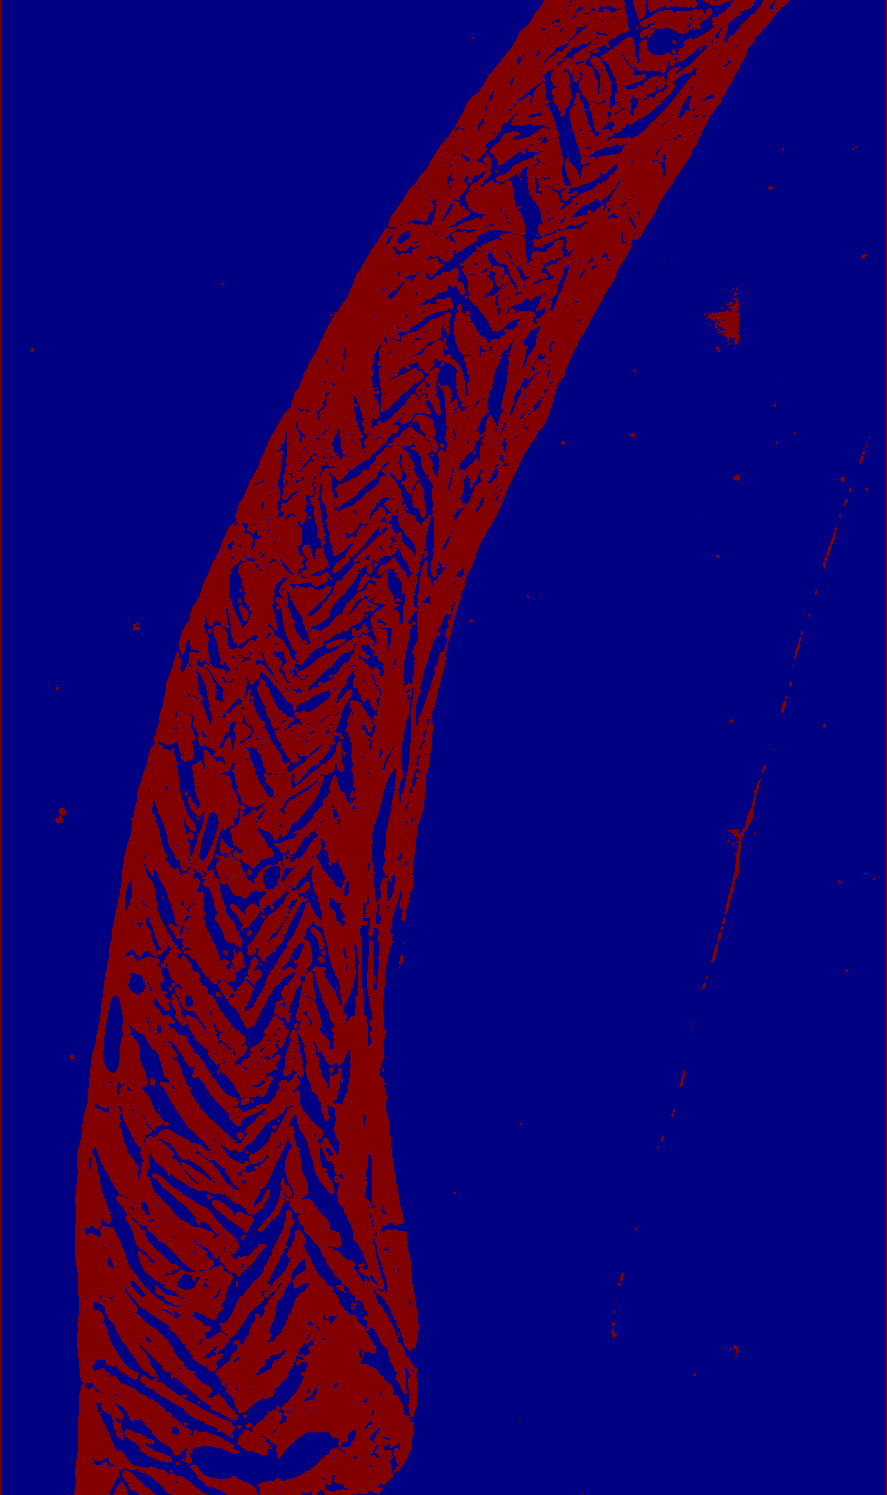
\includegraphics[width=0.24\textwidth]{Ch7/Figs/2D/02_threshold_image.png}}
      \subfigure[][]{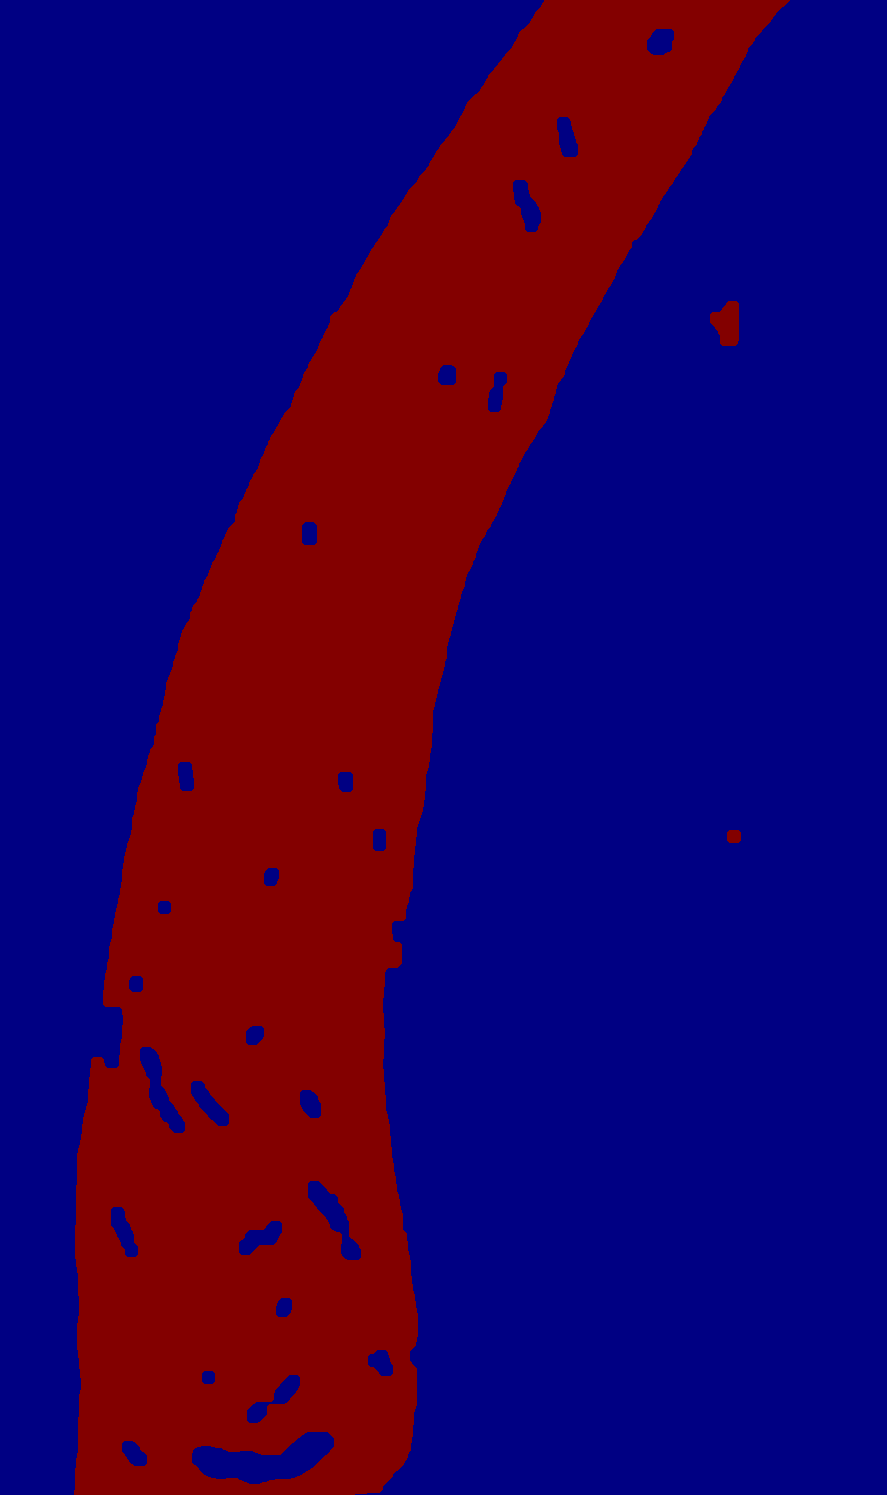
\includegraphics[width=0.24\textwidth]{Ch7/Figs/2D/03_closed_and_opened_threshold_image.png}}
      \subfigure[][]{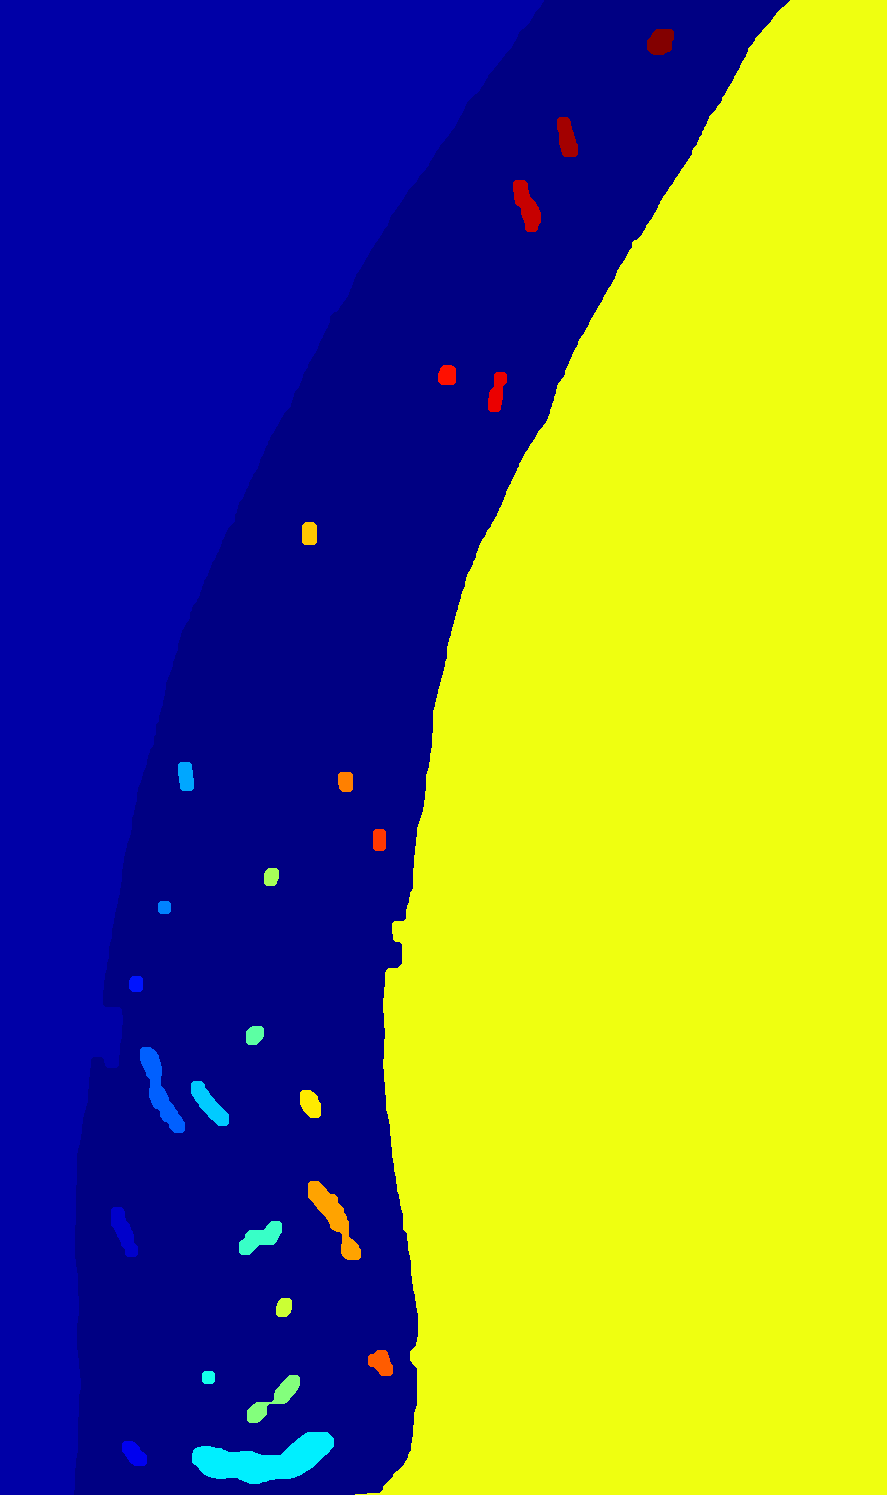
\includegraphics[width=0.24\textwidth]{Ch7/Figs/2D/06_non_tissue_label_image.png}}
      \caption{The highlighted wall segment from Figure~\ref{fig:2D_full_slice} is shown in more detail in \textbf{(a)}. A binary threshold segmentation has been applied in \textbf{(b)}, and morphological opening and closing operations have been applied in \textbf{(c)}, in order to fill small holes and remove small objects. \textbf{(d)} displays an object label image, from which tissue, internal chamber and external cavity regions are manually selected.}
      \label{fig:2D_segmentation}
    \end{figure}
  
    As a proof of concept, we segment the sheet structure and apply the structure tensor to a section of myocardial wall in a single histological slice image, thereby extracting the local in-plane sheet angle across the entire section. Figure~\ref{fig:2D_full_slice} shows the sliver of lower left-ventricular wall that was selected for this purpose from a central rat heart slice. An enlarged view of the sliver is shown in Figure~\ref{fig:2D_segmentation}, along with images of the segmentation process employed to distinguish tissue, chamber and external regions.
  
    It is clear from Figure~\ref{fig:2D_segmentation}~(a) that the myocardial tissue sheets are separated by a great many interstitial clefts, which vary sharply and coherently in direction across the wall. In order to quantify this variation, it is necessary to extract the clefts themselves, and then to measure their orientation relative to the internal and external edges. The long, thin cleft structures must be distinguished from other larger holes in the tissue with no clear angle of orientation, such as myocardial vessels. An overall tissue segmentation has already been manually selected -- as the complement of the two large external blue and internal yellow regions in Figure~\ref{fig:2D_segmentation}~(d). A further threshold segmentation of all near-white pixels is applied, within the overall manual tissue segmentation, and is shown in Figure~\ref{fig:2D_cleft_extraction}~(a). Any region wider than the characteristic width of a cleft is segmented with a morphological opening procedure (Figure~\ref{fig:2D_cleft_extraction}~(b)), and these areas are removed from the original threshold (Figure~\ref{fig:2D_cleft_extraction}~(c)). The structure tensor is calculated at each pixel of the image, and a Gaussian smoothing is applied independently to each of the four scalar elements of the tensor field in order to reduce noise. The orientation at any position within a cleft is then inferred as the direction along the tensor eigenvector associated with the smallest eigenvalue, and thus the lowest intensity gradient.
  
    \begin{figure}[htbp]
      \centering
      \subfigure[][]{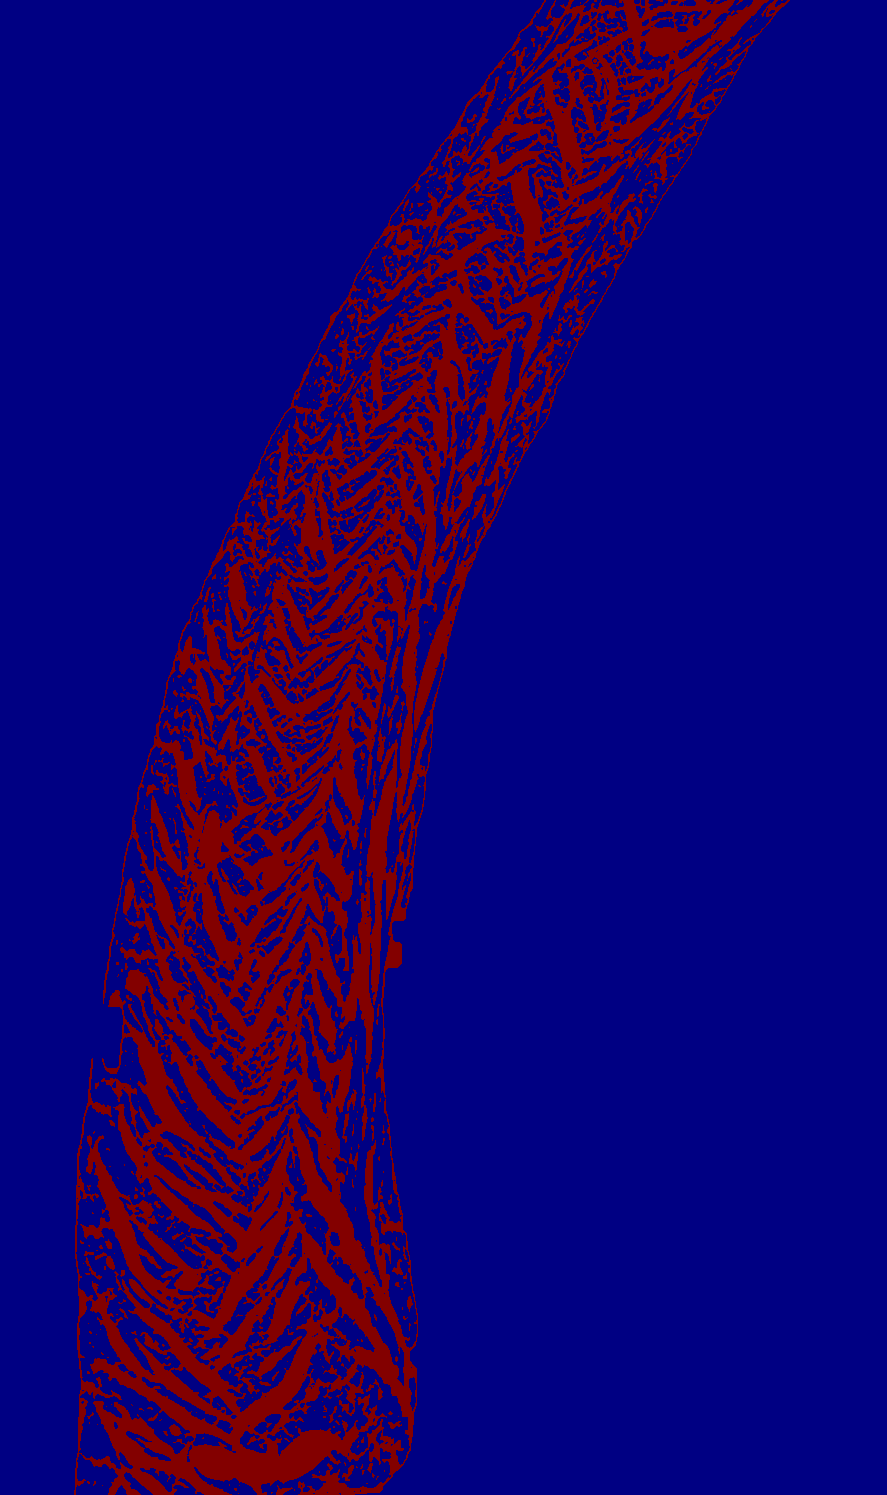
\includegraphics[width=0.24\textwidth]{Ch7/Figs/2D/10_clefts.png}}
      \subfigure[][]{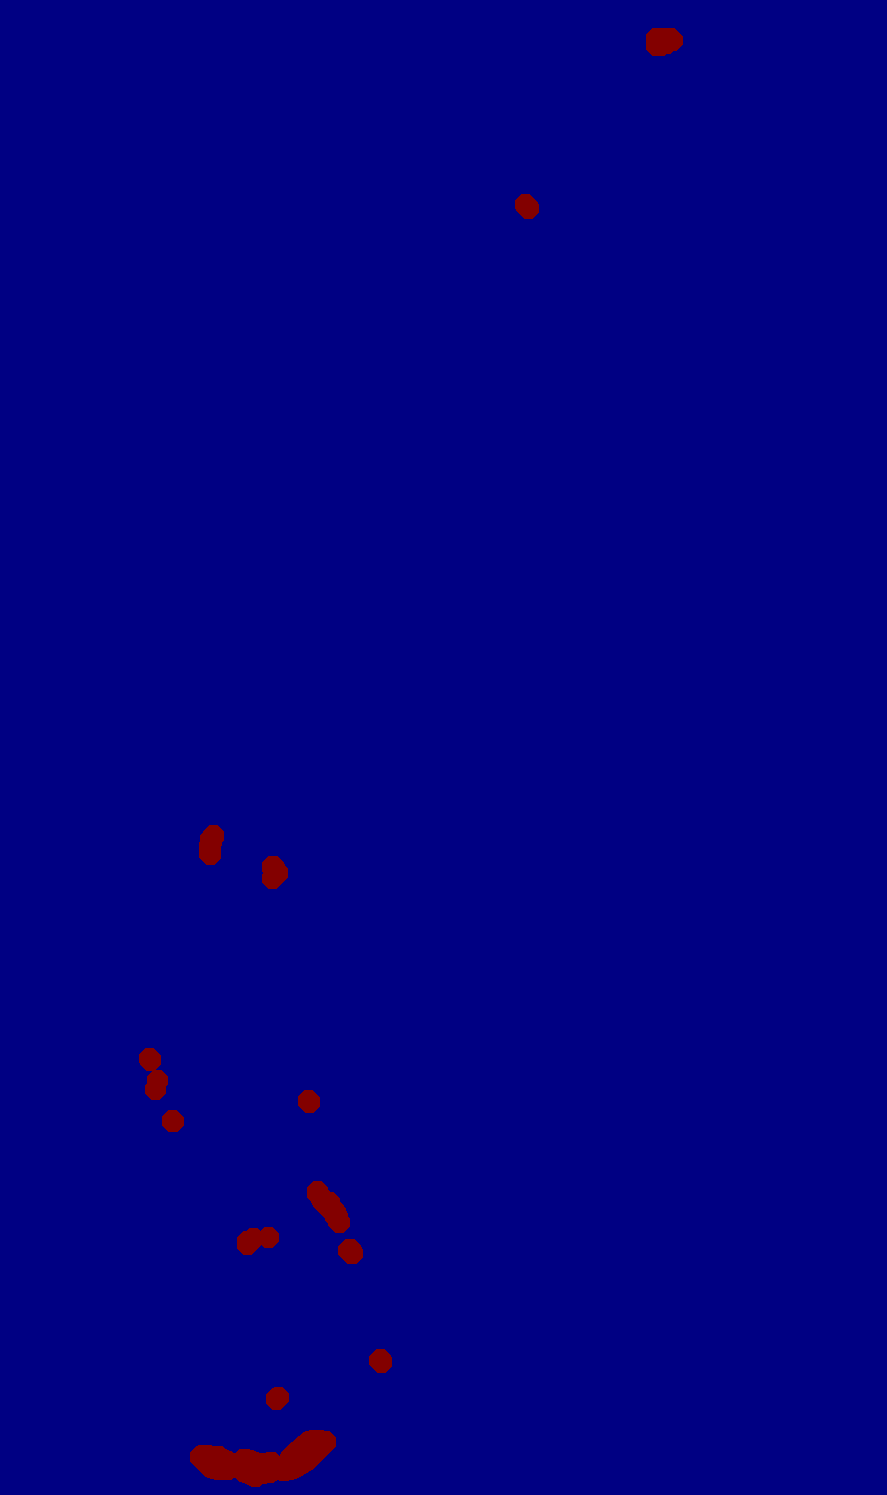
\includegraphics[width=0.24\textwidth]{Ch7/Figs/2D/11_clefts2.png}}
      \subfigure[][]{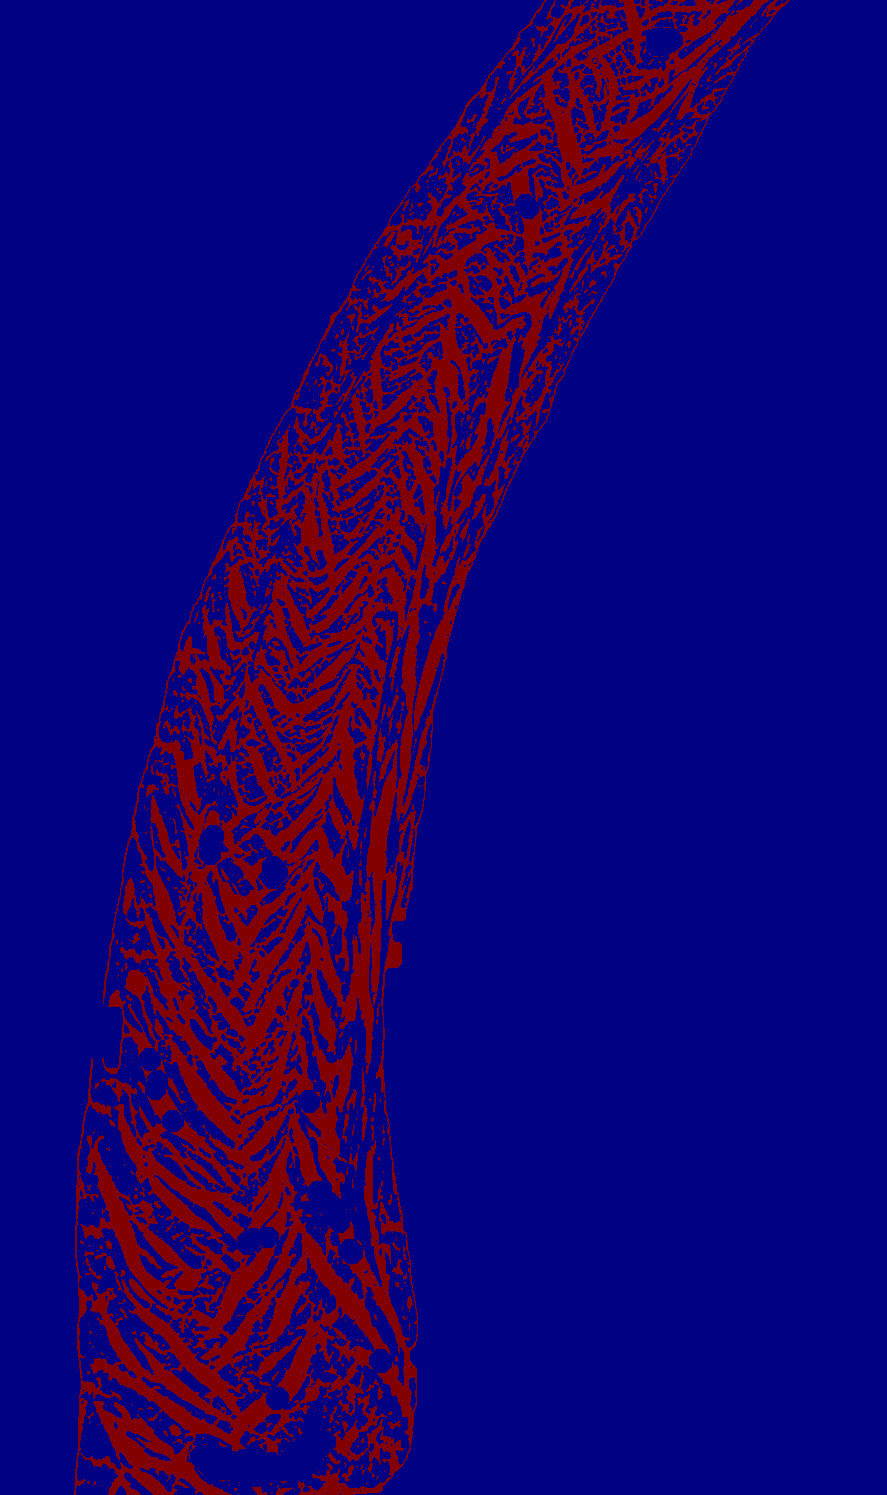
\includegraphics[width=0.24\textwidth]{Ch7/Figs/2D/12_opened_clefts.png}}
      \subfigure[][]{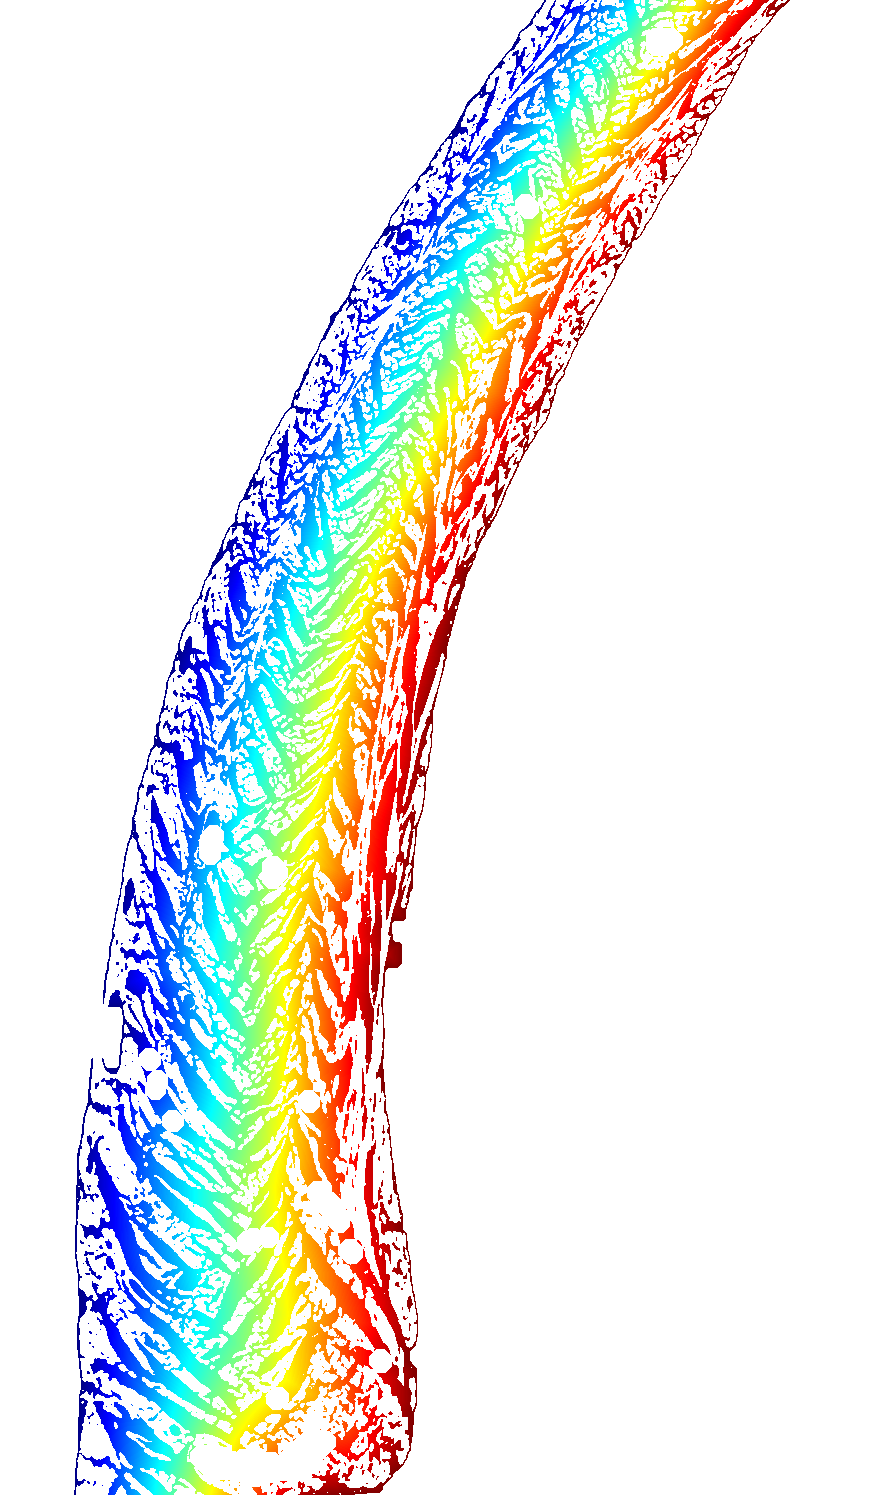
\includegraphics[width=0.24\textwidth]{Ch7/Figs/2D/14_e.png}}
      \caption{A threshold segmentation of all inter-tissue spaces is presented in \textbf{(a)}. Spaces wider than a cleft are determined through the application of an opening filter, of which \textbf{(b)} is the result. These wider spaces are subtracted from the original segmentation in \textbf{(c)}, leaving only the cleft spaces. The normalised distance parameter from endo- to epicardium $e$ is then calculated for each pixel in \textbf{(c)}, plotted as a continuous colourmap in \textbf{(d)}.}
      \label{fig:2D_cleft_extraction}
    \end{figure}
  
    It is conventional in the literature to parameterise the space within the external heart wall with $e$: the normalised relative Euclidian distance from endo- to epicardium. $e$ is defined as zero on the endocardial surface and $1$ on the epicardial surface. It is interesting to explore the relation between $e$ and cleft orientation, and certainly from Figure~\ref{fig:2D_segmentation}~(a), the myocardium appears to be composed of several distinct layers of cleft orientation in a zig-zag pattern, highly coherent within themselves, but sharply angled relative to one another. We apply Euclidian distance transforms to obtain the distances $d_{\text{endo}}$ and $d_{\text{epi}}$ from the internal chamber and the external cavity segmentations, respectively. Armed with the two distances at each pixel, we compute a 2-dimensional value for $e$ throughout the tissue segmentation thusly:
  
    \begin{equation}
      e = \frac{d_{\text{endo}}}{d_{\text{endo}} + d_{\text{epi}} }.
    \end{equation}
  
    A continuous colourmap of the $e$ parameter across the segmented clefts is displayed in Figure~\ref{fig:2D_cleft_extraction}.
    
    All code used to generate figures and calculate sheet angles can be downloaded at \url{http://github.com/mattgibb/sheet-angles}.
  % subsection 2d_slices (end)
  
  \subsection{3D Volumes} % (fold)
  \label{sub:3d_volumes}
    Motivated by the findings from the 2D analysis, we apply the structure tensor to the regionally registered block from Section~\ref{sub:regional_diffusion}. However, before any orientation analysis can be performed, it is crucial to ensure the same sampling rate within the plane of the slices as is between them, so that artificial anisotropy is not introduced. A volume is therefore constructed from slice images that are downsampled and Gaussian smoothed so as to have the same spatial resolution of 10$\mu$m as the slicing. The structure tensor is computed across the isotropic volume, and a Gaussian windowing kernel is then applied to the tensor, with $\sigma$ equal 50$\mu$m.
  
    All the 3D processing code presented here can be obtained at \url{http://github.com/mattgibb/registration}.
  % subsection 3d_volumes (end)
% section methods (end)

\section{Results} % (fold)
\label{sec:results}
  \subsection{2D Slices} % (fold)
  \label{sub:2d_slices}
    
    \begin{figure}[htbp]
      \centering
      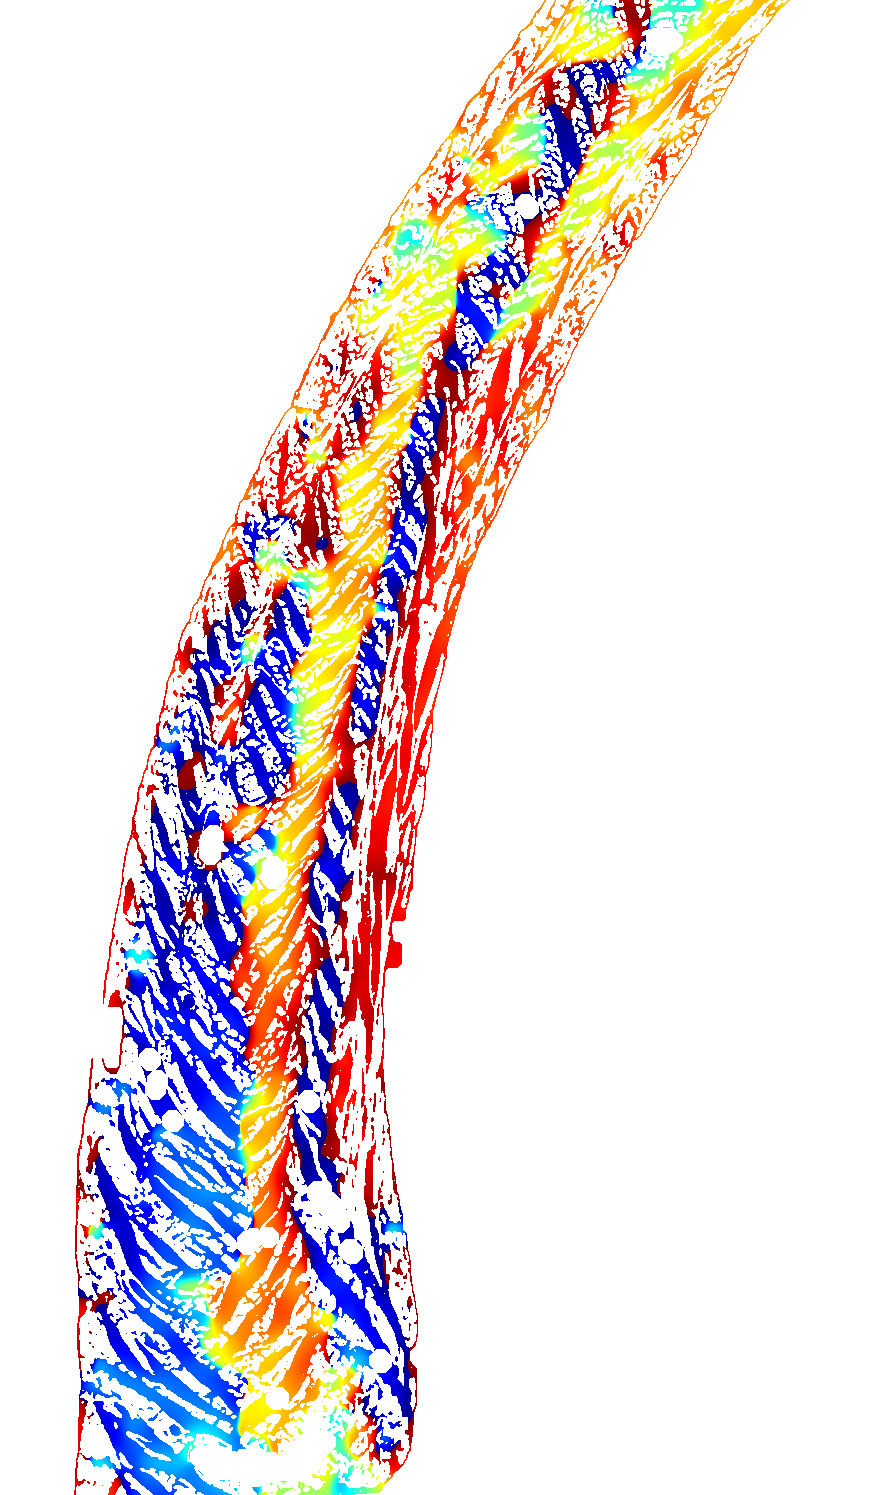
\includegraphics[width=0.8\textwidth]{Ch7/Figs/2D/13_angles.png}
      \caption{A colourmap of the cleft segmentation from Figure~\ref{fig:2D_cleft_extraction}, coloured by the angle of the eigenvector associated with the smallest structure tensor eigenvalue. The results pick out the local orientation very well, with red vertical lines fading with a clockwise rotation into orange, yellow and a horizontal cyan, and finally to a near vertical dark blue between 5 and 11 o'clock.}
      \label{fig:2D_angles}
    \end{figure}
    
    \begin{figure}[htbp]
      \centering
      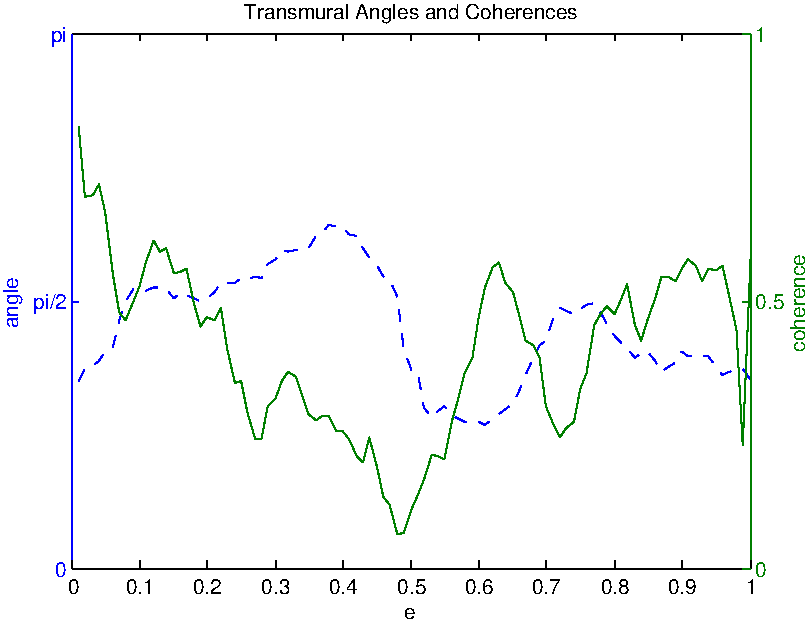
\includegraphics[width=0.8\textwidth]{Ch7/Figs/angles_and_coherences_vs_e}
      \caption{The variation of principal angle and of angular coherence with respect to the transmural parameter $e$. Structure tensors within 100 equispaced bins from $e=0$ to $e=1$ were summed, and the angles plotted are those of the smallest eigenvalue $\lambda_{\text{smaller}}$ with respect to the transmural gradient. The coherences are calculated with the formula $(1 - \lambda_{\text{smaller}}/\lambda_{\text{larger}})^2$.}
      \label{fig:angles_and_coherences_vs_e}
    \end{figure}
    
    The local angle of orientation has been extracted through the application of the structure tensor in Figure~\ref{fig:2D_angles} with prominent success. There is a very clear relationship of the orientation of the extracted clefts to their colouring. The discrete-layered, zig-zagging transmural pattern of cleft orientation has been conspicuously highlighted. Figure~\ref{fig:angles_and_coherences_vs_e} shows the relationship of the average and the spread of transmural angle to the transmural depth. The zig-zagging trend is somewhat reflected here, but unfortunately, the relationship is much less clear, with the low coherence values alluding to a small correlation of $e$ with angle. Referring back to Figure~\ref{fig:2D_angles}, we can see that despite the presence of clear orientational layers, the layers themselves move gradually through the wall from the top to the bottom of the Figure. When the angles are aggregated, therefore, the relationship is obscured.
  % subsection 2d_slices (end)
  
  \subsection{3D volumes} % (fold)
  \label{sub:3d_volumes}
    \begin{sidewaysfigure}[htbp]
      \centering
      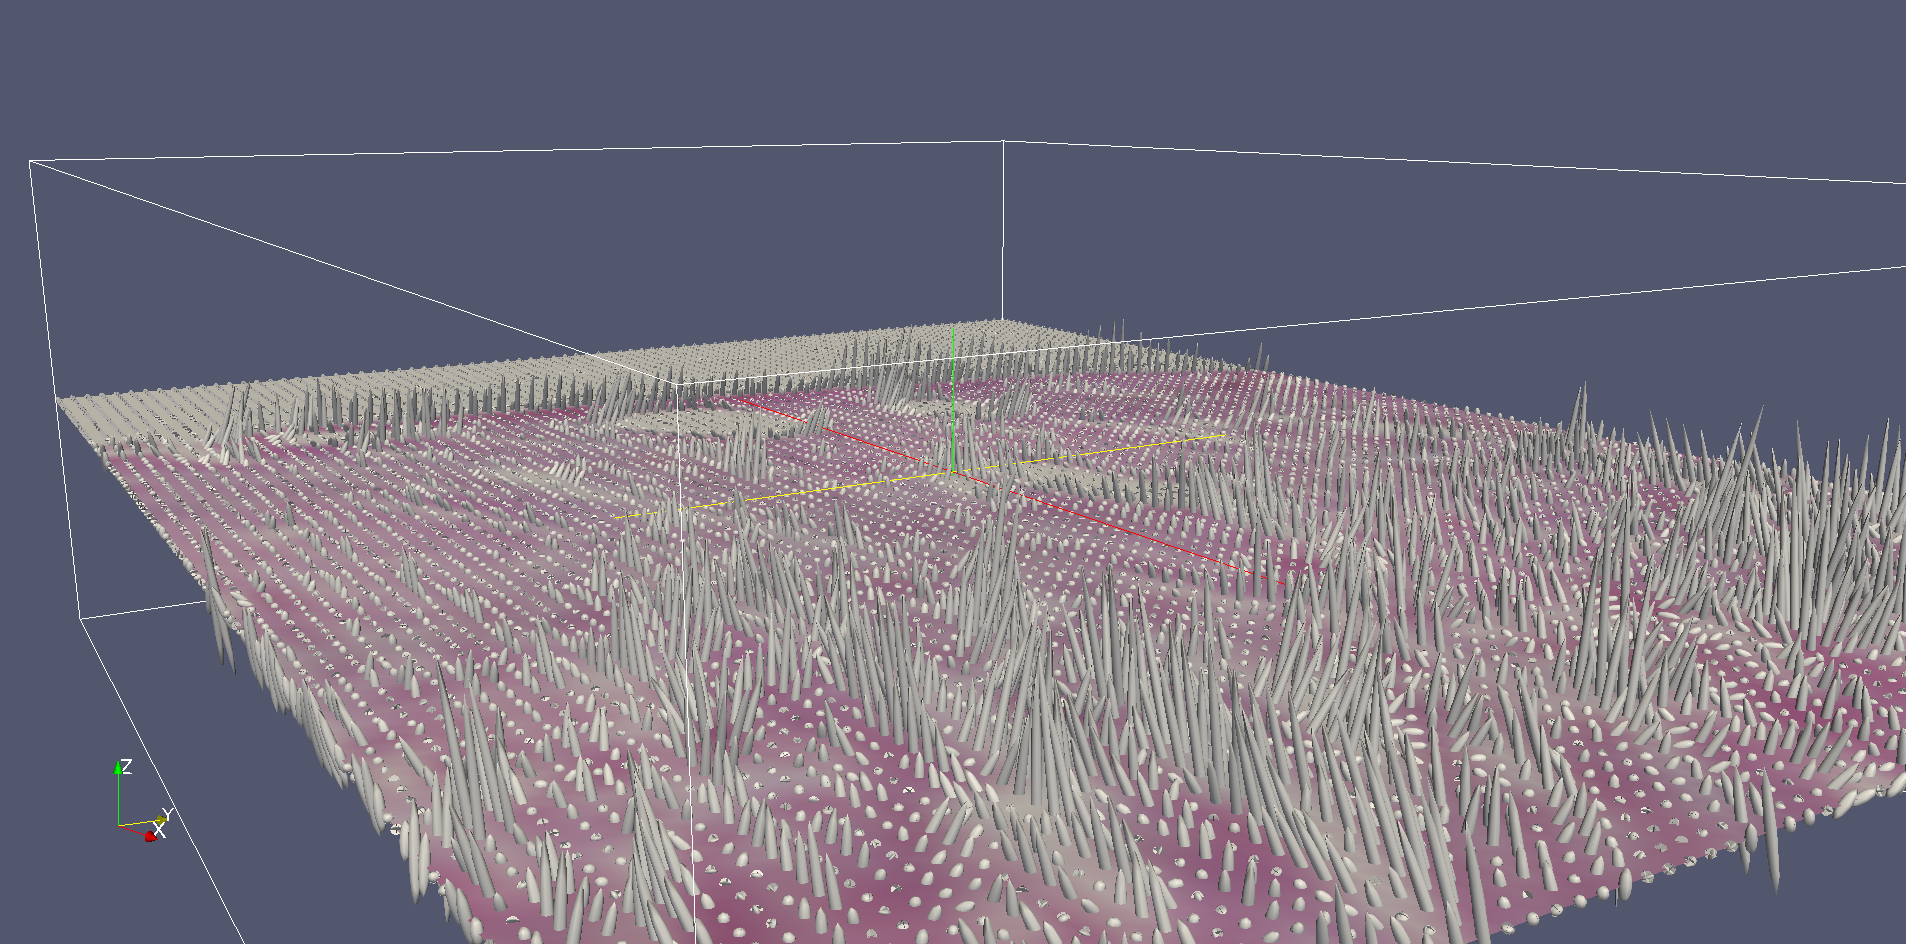
\includegraphics[width=\textwidth]{Ch7/Figs/structure_tensor_glyphs}
      \caption{The central slice through the epicardial vessel region from Section~\ref{sub:regional_diffusion}, overlayed with spheroid glyphs, scaled and oriented by the structure tensor of the pixel intensities. The 2D slice image is presented in Figure~\ref{fig:vessel_cross_section_z}.}
      \label{fig:structure_tensor_glyphs}
    \end{sidewaysfigure}
    
    \begin{sidewaysfigure}[htbp]
      \centering
      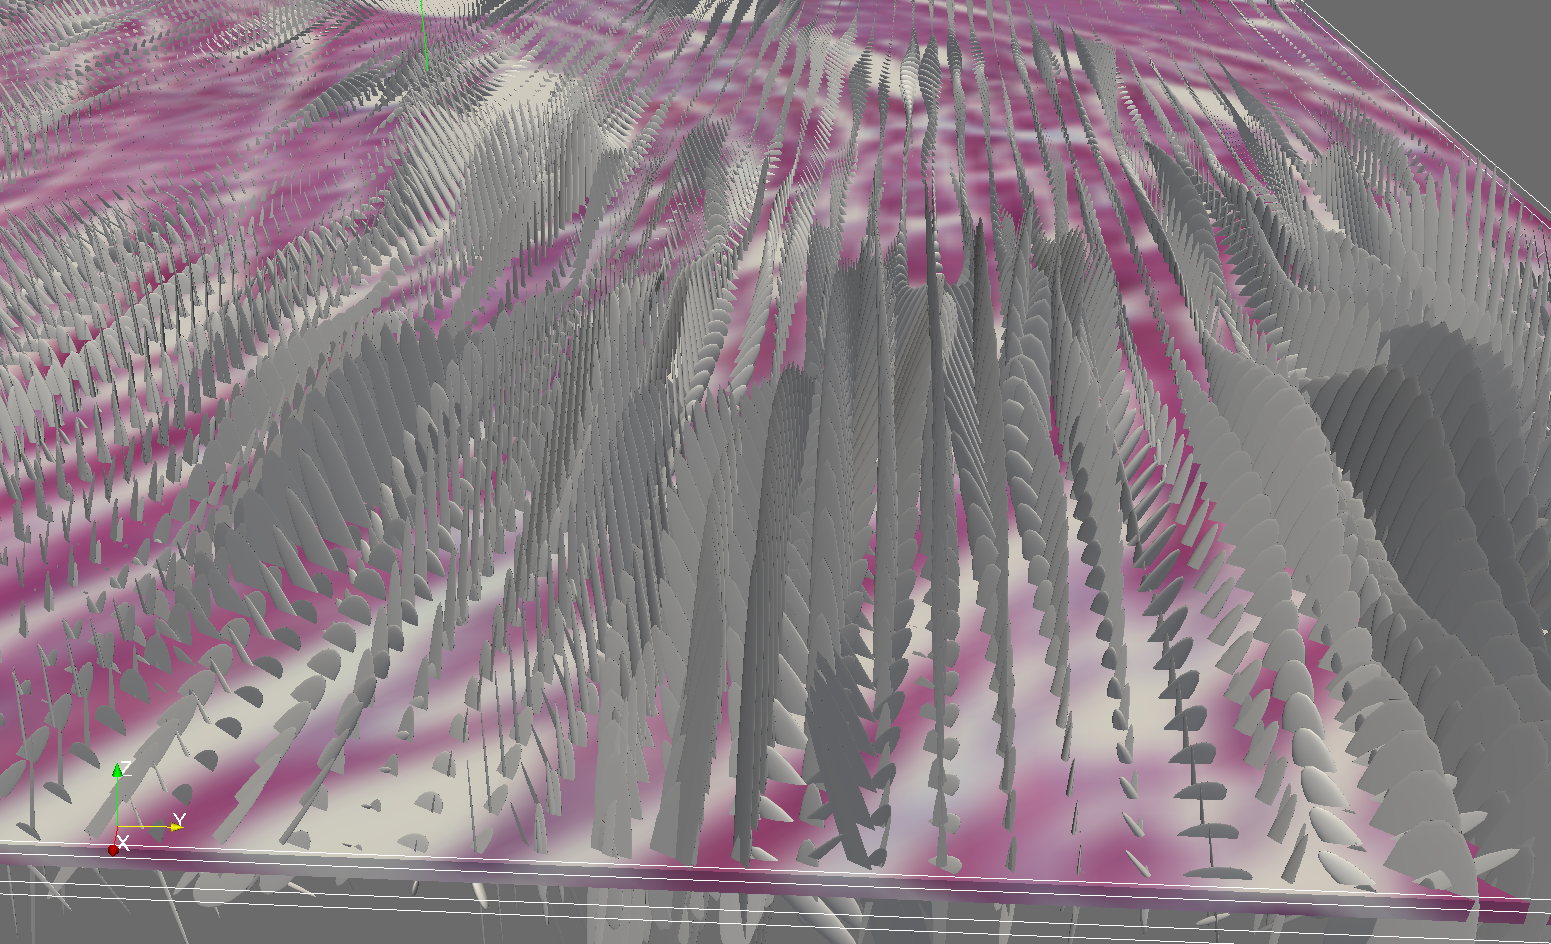
\includegraphics[width=\textwidth]{Ch7/Figs/structure_tensor_glyphs_zoom}
      \caption{A closer view of the lower right hand region of Figure~\ref{fig:structure_tensor_glyphs}, where the individual shape of the spheroid glyphs are made clearer.}
      \label{fig:structure_tensor_glyphs_zoom}
    \end{sidewaysfigure}
    
    \begin{figure}[htbp]
      \centering
      \subfigure[][x]{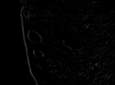
\includegraphics[width=0.45\textwidth]{Ch7/Figs/x_eigencomponent.png}}
      \subfigure[][y]{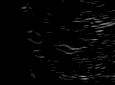
\includegraphics[width=0.45\textwidth]{Ch7/Figs/y_eigencomponent.png}}
      \subfigure[][z]{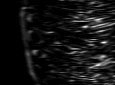
\includegraphics[width=0.45\textwidth]{Ch7/Figs/z_eigencomponent.png}}
      \subfigure[][combined]{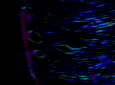
\includegraphics[width=0.45\textwidth]{Ch7/Figs/rgb_eigencomponents.png}}
      \caption{\textbf{(a)}, \textbf{(b)} and \textbf{(c)} map the absolute magnitudes of the x-, y- and z- components of the largest eigenvector of the structure tensor, of the same central slice from Figure~\ref{fig:structure_tensor_glyphs}. The volumewise maximums for the x-, y-, and z- components were 15.4, 39.9 and 70.1, respectively; the intensities have thus been scaled from 0 (black) to 70.1 (white). \textbf{(d)} combines the intensities in an RGB image, with red x, green y and blue z.}
      \label{fig:eigencomponents}
    \end{figure}
    
    Figures~\ref{fig:structure_tensor_glyphs} and \ref{fig:structure_tensor_glyphs_zoom} illustrate the form of the structure tensor across the central histological slice of the epicardial block. A regular grid of spheroid glyphs are plotted at each pixel of the slice, with principal axes aligned and proportional to the eigenvectors and eigenvalues of the structure tensor. It is evident that the largest tensors are, as expected, javelin-like, as one eigenvalue greatly exceeds the other two perpendicular to the clefts. It is also evident that larger tensors are oriented predominantly in the z-direction perpendicular to the plane, a phenomenon that increases visibly with distance from the epicardial wall. Figure~\ref{fig:eigencomponents} echoes these findings, showing grayscale images of the magnitudes of the three components of the largest eigenvector. By far the brightest image is that of the z-component. This dominance is also expressed in the largely blue appearance of Figure~\ref{fig:eigencomponents} (d), with only small tinges of red and green. Unfortunately in this case, even extremely small displacements of the slices relative to each other has been enough to drown the gradient signal from the fibre direction.
  % subsection 3d_volumes (end)
  
% section results (end)

\section{Discussion} % (fold)
  We have outlined a method for the extraction of microstucture from high resolution histological images, and demonstrated its application on both 2-dimensional slices and registered tissue volumes. We have encountered a high level of organised layered structure, and have made way towards quantifying the relationship between angle and transmural position. We have established that the success of this quantification depends on the choice and size of region, through the presence or absence of slowly-varying transmural meandering of the discrete layers. We have made progress towards characterising this layered structure in 3 dimensions, and shown that very tiny aberrations in the tissue images and positions contribute a considerable level of noise in this regard. If this noise can be ameliorated, then intricate microstructure can be resolved.
  
  In developing the 2-dimensional techniques, we surveyed 40 central slices from 2 rat hearts in 4 separate regions: the upper and lower free wall of the left ventricle, and the upper and lower septum. It was found that local sheet orientation was resolved well in almost all regions. Lamentably however, in the large majority of cases, the results suffered from the same aggregation problems manifest in Figure~\ref{fig:angles_and_coherences_vs_e} and were too blurred to draw reasonable conclusions from, as layers meandered intramurally across a range of $e$ values.
  
  In the 3D volume, the dominance of intensity gradient in the z-direction is a result of very small internal distortions, discontinuities and fractures within slices not represented by the affine transformations. Unfortunately, the misalignment often leads to a `zig-zagging' of intensities perpendicular to the slices and at the frequency of the slicing, which manifests as an inflated z-gradient. There are a number of things which can be explored to correct for this z-dominance. Experimentation with a range of edge-preserving smoothing filters, configured so that the gradient components in all directions are approximately similar, may well provide stronger feature extraction. 
\label{sec:discussion}
  
% section discussion (end)

% chapter extraction_of_3d_anatomical_structure (end)
